% !TeX root = ../../thesis.tex

\chapter{Code Division Multiple Access}
\label{chp:cdma}

\todo{Should I explain differences TDM/FDM/CDMA ??}


Each LED requires a unique ID.
When the LEDs are modulating to transmit their IDs, the current of multiple LEDs are aggregated.
The aggregated current will flow through the smart-meter, in other words, the only information the  smart-meter has, is the aggregated current.
And from these aggregated IDs, the smart-meter should be able to identify which IDs are present.
If it can do that, the smart-meter is able to tell which LEDs are on and which or off.

This chapter will explain how these IDs can be constructed by using CDMA codes.
To see which codes are the best, first the performance metrics are explained.
Then several codes will be discussed and the performance metrics for each code will be highlighted.
Finally the codes will be compared to each other.



% !TeX root = ../../thesis.tex

\section{Performance Metrics of a CDMA Sequence}
\label{sec:performance-metrics-cdma}

To be able to objectively determine which code sequence is the best for certain environments, metrics are needed to compare the performance of a sequence.
Such metrics are: auto- and cross-correlation, length of the code and how many unique codes can be produced which are in the same set, meaning with the same length, so that they can be used together in the same system.
Also if the codes can be used in a synchronous only or in an a-synchronous environment has to be considered.


Correlation is a measure for determining how much sequence $X$ is similar to sequence $Y$ and can be found in \autoref{eq:correlation}.
With $L$ being the length of the code and $\tau$ the time-shift.
When sequence $X$ and $Y$ are the same sequence, we speak of the autocorrelation.
When they are two different sequences, we speak of the cross-correlation. 

\begin{equation}
	R(\tau)_{xy} = \displaystyle\sum_{i = 0} ^ {L - 1} x(i) \times y(i + \tau) {\text{  with $\tau = 0, 1, 2, \dotsc, L$}}
	\label{eq:correlation}
\end{equation}


%commented out because this will never be used and therefor only adds unnecessary text

%Another way to calculate the correlation between two sequences is to count the number of agreements and disagreements between the two sequences, see \autoref{eq:correlation-a-d}, this comes in handy when comparing two digital sequences, which both have $0$ and $1$ signal levels.

%\begin{equation}
%	R(\tau) = \text{\# of agreements} - \text{\# of disagreements} 
%	\label{eq:correlation-a-d}
%\end{equation}




The properties of an ideal set of codes should be, that the autocorrelation for each code in the set should be $0$ for each time-shift $\tau \neq 0$, at $\tau = 0$ the autocorrelation should be $L$, this value would than be a peak value for which we can identify if this code is present in the received signal.
If the signal is the sampled current and the code is the ID of a LED, then we can say the LED is on when the auto-correlation peak is seen.
The ideal cross-correlation properties should be $0$ for every time-shift $\tau$, so that no code interferes with any other code, hereby causing no MAI (Multiple Access Interference).



The length of a code is also of importance, because each chip of the code has to be transmitted.
Assuming a constant modulating frequency, the time it takes to transmit a code sequence is proportional to the length of that code sequence.
The length of the code will also determine, to some extent, the number of codes in the same set.
The number of codes in the same set determines the scalability of the system.






% !TeX root = ../../thesis.tex

\section{Code Sequences}
\label{sec:code-sequences}

In this section different code sequences will be explained.
Their performance will be stated by the metric detailed in \autoref{sec:performance-metrics-cdma}.
Finally a comparison between the sequences is made.



% !TeX root = ../../../thesis.tex

\subsection{Orthogonal Sequences}
\label{subsec:orthogonal-sequences}

Orthogonal sequences, also known as Walsh-Hadamard sequences, are sequences which are created using a Hadamard matrix.
Hadamard matrices are square $n \times n$ matrices which are recursively generated.
Starting with a $1 \times 1$ matrix: 
		$H_{1} = \begin{bmatrix} 1 \end{bmatrix}$, then 
		$H_{2} = \begin{bmatrix} 1 & 1 \\ 1 & -1 \end{bmatrix}$.
See \autoref{eq:hadamard-matrix-creation} for a general recursive formula to generate other ranks of Hadamard matrices \cite{714616}.

\begin{equation}
	H_{2n} = 
	\begin{bmatrix} 
		H_n & H_n \\ 
		H_n & -H_n 
	\end{bmatrix}
	\label{eq:hadamard-matrix-creation}
\end{equation}

The matrix can also be filled with binary values: $0$ and $1$. In that case the general recursive formula is stated in \autoref{eq:hadamard-matrix-creation-bin}. 

\begin{equation}
	H_{2n} = 
	\begin{bmatrix} 
		H_n & H_n \\ 
		H_n & \overline{H_n}
	\end{bmatrix}
	\label{eq:hadamard-matrix-creation-bin}
\end{equation}




The Hadamard matrix has the property that every row in the matrix, apart from the first row, is orthogonal to every other row, meaning that the cross-correlation is zero.
And apart from the first row, all other rows have the exact same number of $+1$s and $-1$s, meaning that the codes are balanced.

Hadamard matrices exist for every power of $2$, so the code length is also a power of $2$.
For $\tau = 0$, the cross-correlation is $0$, but when $\tau \neq 0$ not all the rows have a zero cross-correlation with all other rows.
All rows of the matrix have the property that the auto-correlation at $\tau = 0$ is equal to $L$.
But when $\tau \neq 0$, undesirable behavior occurs as can be seen in \autoref{fig:autocorr-hadamard}.
The autocorrelation function has several high peaks where only one is desired, namely at $\tau = 0$.
This means that if an LED starts modulating its code, but the smart-meter does not know when in time the start of this code is, the smart-meter will get false-positives for data.
If there was a way that the smart-meters and all the LEDs could be synchronized with each other, the orthogonal codes will work.

\begin{figure}[t]
	\centering
	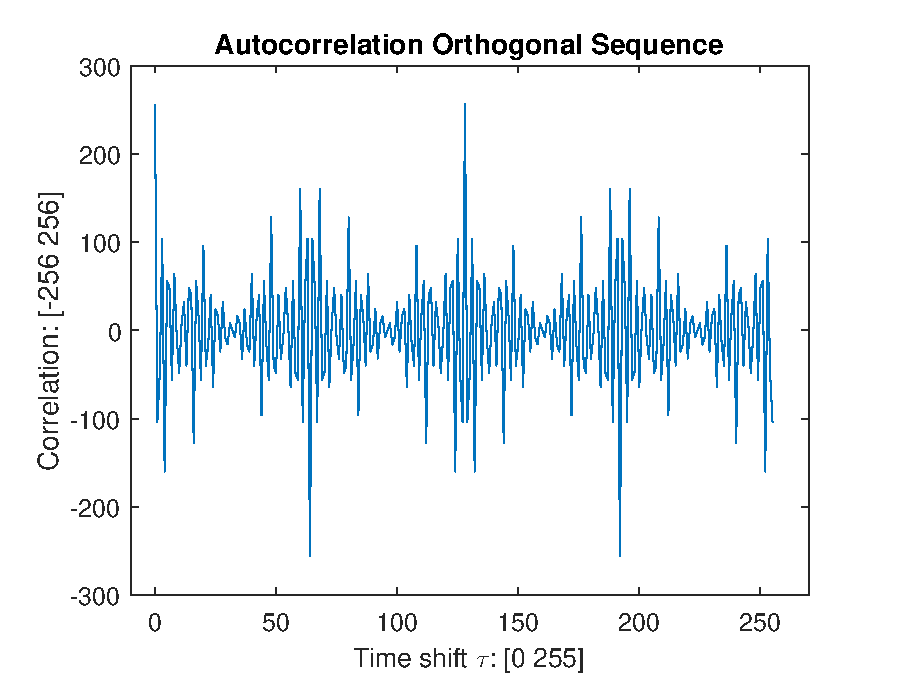
\includegraphics[width=\textwidth]{chapters/cdma-chapters/codes/autocorr-hadamard.eps}
	\caption{Autocorrelation of orthogonal sequence with row index 120 of length 256.}
	\label{fig:autocorr-hadamard}
\end{figure}





To conclude: the entire set of orthogonal codes of length $L$, has $L - 1$ codes in the set which does make it a scalable set.
But the auto- and cross-correlation only have the desired properties when the codes are sent synchronously. 




\subsubsection{Cyclically Orthogonal Walsh Hadamard Codes}

To overcome the problem when sending orthogonal codes in an asynchronous manner, a subset of the orthogonal codes have been identified that are still orthogonal to each other, no matter how these codes are time-shifted with respect to each other.

In \cite{1182447} the authors proved that an Hadamard matrix of size $2^P$ could be divided into $P + 1$ subsets of rows, where one row could be selected giving $P + 1$ orthogonal rows for each time-shift $\tau$.
In other words, this subset of rows have a cross-correlation of zero, for every time-shift $\tau$.
These codes are called Cyclically Orthogonal Walsh Hadamard Codes (COWHC).
With code length $L$ there are $\log_2 L$ codes in the set, which makes these codes not scalable \cite{1182447}. 
Also the auto-correlation does not have a clear peak to identify the code, because these codes are an unmodified subset of the original orthogonal sequences.
For these sequences the auto-correlation has already been shown in \autoref{fig:autocorr-hadamard}.

These codes suffer from the same auto-correlation problems as the normal Orthogonal codes as described in \autoref{subsec:orthogonal-sequences} and they have the additional drawback that they are less scalable.

% !TeX root = ../../../thesis.tex

\subsection{Pseudorandom Noise Sequences}
\label{subsec:pn-sequences}

The main drawback with the orthogonal codes, was that these codes cannot be used in an asynchronous manner.
To overcome this drawback, PN sequences were investigate which can be used in an asynchronous manner.

PN sequences are sequences which look like they are randomly generated but they are easily generated in software or hardware.
They are generated with linear shift registers of length $n$.
The sequences have the following noise-like properties~\cite{mitra2008pseudo}:

\begin{itemize}
	\item Balance property:	Any PN sequence of length $L = 2^n - 1$ contains exactly $2^{n-1}$ ones and exactly $2^{n-1} - 1$ zeros.

	\item Runs property: A run is a subset of the sequence where all the consecutive numbers are the same. In any PN sequence, $1/2$ of the runs have length 1, $1/4$ have length 2, $1/8$ have length 3 and so on.

	\item Auto-correlation property: The auto-correlation function of a PN sequence will take on two values as can be seen in \autoref{eq:autocorr-pn} and \autoref{fig:autocorr-pn}.


\end{itemize}






\begin{equation}
	\label{eq:autocorr-pn}
	R(\tau) = 
		\begin{cases}
			L    & \quad \text{if } \tau = 0 \\
			-1   & \quad \text{if } \tau \neq 0 \\
		\end{cases}
\end{equation}






\begin{figure}[t]
	\centering
	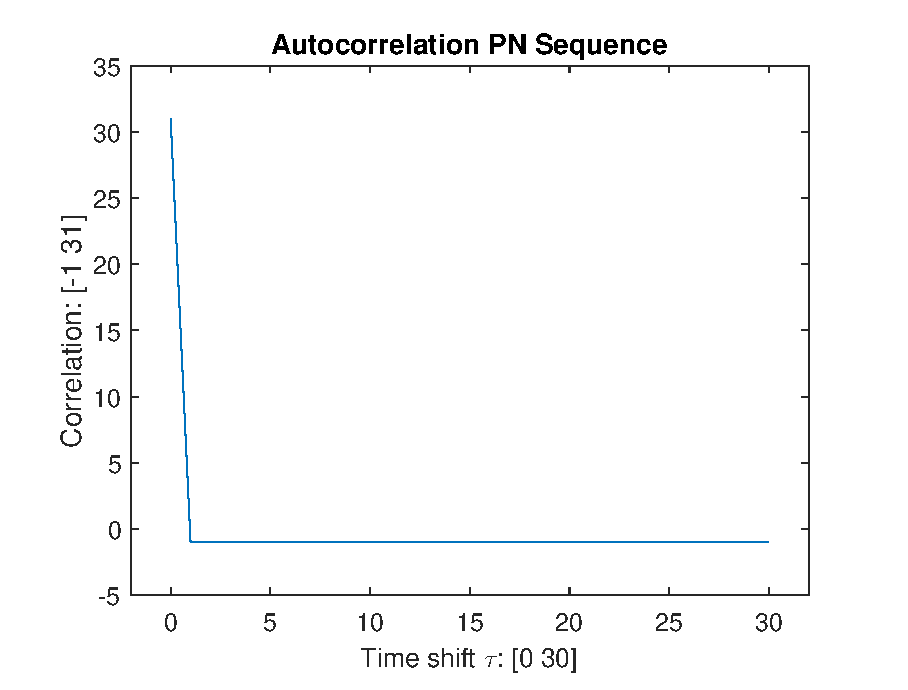
\includegraphics[width=\textwidth]{chapters/cdma-chapters/codes/autocorr-pn.eps}
	\caption{Autocorrelation of PN sequence of length 31.}
	\label{fig:autocorr-pn}
\end{figure}





PN sequences are generated using a linear feedback shift register (LFSR) \cite{Wang:1988:LFS:52007.52024}.
\autoref{fig:lfsr} shows an $n$ length LFSR with XOR gates attached to each element of the register and a feedback loop into the last element. 
The LFSR is defined entirely by the feedback function, also called a characteristic polynomial.
It determines the length and the type of sequence generated.
The polynomial looks like \autoref{eq:lfsr-polynomial}.
For example: Given a polynomial $q(x) = x^5 + x^2 + 1$, tells us that the LFSR has length $5$ and that the outputs of elements with number zero and two are XORed and fed back into the last element. 

\begin{equation}
	\label{eq:lfsr-polynomial}
	p(x) = x^n + C_{n-1} x^{n-1}  + C_{n-2} x^{n-2} + \dotsc + C_{2} x^{2}  + C_{1} x  + C_{0}
\end{equation}

\begin{figure}[t]
	\centering
	\begin{tikzpicture}


		\node[block                  ] (last_register) {$s_{n-1}$};
		\node[block, right = 1cm of last_register] (second_last_register) {$s_{n-2}$};
		\draw[line] (last_register.east) -- (second_last_register.west) ;

		\node[block, right = 3cm of second_last_register] (second_register) {$s_{1}$};
		\node[block, right = 1cm of second_register] (mid_register) {$s_{0}$};
		\draw[line] (second_register.east) -- (mid_register.west) ;

		\draw[dashed, line] (second_last_register.east) -- (second_register.west) ;

		\node[coordinate, right = 2cm of mid_register] (output_point) {};
		\draw[line] (mid_register.east) -- (output_point.west) node [midway, above] {output};

		\node[XOR, scale=2, below = 2cm of second_register] (first_xor) {};
		\draw[line] (second_register.south) -- (first_xor.north) node [midway, right] {$C_1$};
		\draw[line] (mid_register.south) |- (first_xor.east) node [pos=0.21, right] {$C_0$};

		\node[coordinate, right = 1.5cm of second_last_register] (h) {};
		\node[XOR, scale=2, below = 2.5cm of h] (mid_xor) {};
		\draw[line] (first_xor.west) -- (mid_xor.east) ;
		\draw[dashed, line] (h.south) -- (mid_xor.north) ;

		\node[XOR, scale=2, below = 2cm of second_last_register] (second_last_xor) {};
		\node[XOR, scale=2, below = 2cm of last_register] (last_xor) {};

		\draw[line] (second_last_register.south) -- (second_last_xor.north) node [midway, right] {$C_{n-2}$};
		\draw[line] (mid_xor.west) -- (second_last_xor.east) ;
		
		\draw[line] (second_last_xor.west) -- (last_xor.east) ;
		\draw[line] (last_register.south) -- (last_xor.north) node [midway, right] {$C_{n-1}$};

		\node[coordinate, left = 1cm of last_register] (return_point) {};
		
		\draw[line] (last_xor.west) -| (return_point) -- (last_register.west) ;




	\end{tikzpicture}
	\caption{Linear feedback shifter register of length $n$, with XOR gates, to produce a PN sequence.}
	\label{fig:lfsr}
\end{figure}


For PN sequences, there exists no formula for the cross-correlation of two different PN sequences. 
Exhaustive analysis is required to find out which sequences or entire sets have the cross-correlation characteristics that are good enough for the user's application.
In \autoref{tbl:pn-sequences-C-and-cross-corr} the calculated peak cross-correlations per PN sequences from the same set can be found.
For each sequence the cross-correlation is calculated with every other sequence for every time-shift $\tau$. 
Then the maximum of those cross-correlation is taken and used for the peak cross-correlation.
For the PN codes the auto-correlation does not have to be calculated, this is already shown in \autoref{eq:autocorr-pn}.



The size of the code set is limited.
For a LFSR with $n$ registers, the maximum number of possible codes $C$ is given by \autoref{eq:num-of-pn-codes} \cite{mutagi1996pseudo}, where $P_i$ are the prime factors of $2^n - 1$ and $\alpha_i$ is the power of $i$th prime factor.

\begin{equation}
	\label{eq:num-of-pn-codes}
	C = \frac{1}{n} \prod \{ P_{i} ^ {(\alpha_i - 1)} \times (P_i - 1) \}
\end{equation}

For example when using a LFSR of size $n = 6$, $2^n - 1 = 63$, which can be factored into $3^2 \times 7$.
Giving $P_1 = 3$, $P_2 = 7$, $\alpha_1 = 2$ and $\alpha_2 = 1$.
Thus, the maximum number of codes is: $C = \frac{1}{6} \times \{ 3^{2 - 1} \times (3 - 1) \} \times \{ 7^{1 - 1} \times (7 - 1) \} = 6$.
Another example: Say there are going to be 144 LEDs, so 144 codes are needed. 
This means a code length of 4095 chips.
For PN sequences of other lengths, see \autoref{tbl:pn-sequences-C-and-cross-corr} for the number of codes.


\begin{table}[tbp]
	\centering
	\begin{tabular}{  | l | l | l | }

		\hline
		Code Length (L)	& Number of Codes (C) 	& Peak cross-correlation	\\ \hline
		
		7				& 2						& 5						\\ \hline					
		15				& 2						& 9						\\ \hline			
		31				& 6						& 11					\\ \hline			
		63				& 6						& 23					\\ \hline		
		127				& 18					& 41					\\ \hline		
		255				& 16					& 95					\\ \hline	
		511				& 48					& 113					\\ \hline	
		1023			& 60					& 383					\\ \hline		
		2047			& 176 					& 287					\\ \hline		
		4095			& 144					& 144					\\ \hline		


	\end{tabular}
	\caption{Table showing the number of PN sequences of the same length along with the peak cross-correlation \cite{kettunen1997code}. }
	\label{tbl:pn-sequences-C-and-cross-corr}

\end{table}


To conclude: PN sequences have less number of sequences in the same set, compared to orthogonal sequences, so they are less scalable.
But the PN sequences can be used in an asynchronous manner, with good auto-correlation.
But the cross-correlation properties causes interference, which limits the amount of transmitters that can transmit concurrently.












% !TeX root = ../../../thesis.tex

\subsection{Gold Sequences}
\label{subsec:gold-sequences}

The PN sequences gives us a set of codes which is not scalable and suffers from interference issues, but it can work in an asynchronous environment.
To solve these issues, Gold codes were investigated.

Gold sequences are a type of PN sequence.
%These codes are used for as C/A Code (Coarse Acquisition) in GPS satellites \cite{gold-in-sats}. 
They are created by using two LFS registers as shown in \autoref{fig:gold-lfsr}.
In this figure there are two vectors $s$ and $t$ and two polynomials $C$ and $D$.
For a sequence to be constructed in this way that is a Gold sequence, only preferred pairs of polynomials can be used \cite{kedia2012comparative}.
Only preferred pairs of polynomials will yield a set of codes that will have a three valued cross-correlation function.
A method for selecting these preferred pairs of polynomials can be found in \cite{1054106}.
The polynomials are the same as explained for the PN sequences.
For example, $p(x) = x^3 + x^2 + 1$ and $q(x) = x^3 + x + 1$ are a preferred pair and can be used with two LFS registers of length $3$ in a construction as shown in \autoref{fig:gold-lfsr}.
When we have the polynomials $p(x)$ and $q(x)$, which are a preferred pair and produce the PN sequences $d_1$ and $d_2$ respectively, the resulting set of Gold codes is defined as can be seen in \autoref{eq:gold-def}, where $T^k$ represent the cyclic shift of $k$ bits.

\begin{equation}
	\label{eq:gold-def}
	Gold(d_1, d_2) = \{ d_1, d_2, d_1 \oplus d_2, d_1 \oplus Td_2, d_1 \oplus T^2d_2, \dotsc, d_1 \oplus T^{L - 1}d_2 \}
\end{equation}


\begin{figure}[t]
	\centering
	\begin{tikzpicture}

		\node[block                  ] (last_register1) {$s_{n-1}$};
		\node[block, right = 1cm of last_register1] (second_last_register1) {$s_{n-2}$};
		\draw[line] (last_register1.east) -- (second_last_register1.west) ;

		\node[block, right = 3cm of second_last_register1] (second_register1) {$s_{1}$};
		\node[block, right = 1cm of second_register1] (mid_register1) {$s_{0}$};
		\draw[line] (second_register1.east) -- (mid_register1.west) ;

		\draw[dashed, line] (second_last_register1.east) -- (second_register1.west) ;

		\node[coordinate, right = 1cm of mid_register1] (output_point1) {};

		\node[XOR, scale=2, above = 2cm of second_register1] (first_xor1) {};
		\draw[line] (second_register1.north) -- (first_xor1.south) node [midway, right] {$C_1$};
		\draw[line] (mid_register1.north) |- (first_xor1.east) node [pos=0.21, right] {$C_0$};

		\node[coordinate, right = 1.5cm of second_last_register1] (h1) {};
		\node[XOR, scale=2, above = 2.5cm of h1] (mid_xor1) {};
		\draw[line] (first_xor1.west) -- (mid_xor1.east) ;
		\draw[dashed, line] (h1.north) -- (mid_xor1.south) ;

		\node[XOR, scale=2, above = 2cm of second_last_register1] (second_last_xor1) {};
		\node[XOR, scale=2, above = 2cm of last_register1] (last_xor1) {};

		\draw[line] (second_last_register1.north) -- (second_last_xor1.south) node [midway, right] {$C_{n-2}$};
		\draw[line] (mid_xor1.west) -- (second_last_xor1.east) ;
		
		\draw[line] (second_last_xor1.west) -- (last_xor1.east) ;
		\draw[line] (last_register1.north) -- (last_xor1.south) node [midway, right] {$C_{n-1}$};

		\node[coordinate, left = 1cm of last_register1] (return_point1) {};
		
		\draw[line] (last_xor1.west) -| (return_point1) -- (last_register1.west) ;

		%%%%%%%%%%%%%%%%%%%%%%%%%%%%%%%%%%%%%%%%%%%%%%%%%%%%%%%%%%%%%%%%%%%%%%%%%%%%


		\node[block, below = 2cm of last_register1] (last_register) {$t_{n-1}$};
		\node[block, right = 1cm of last_register] (second_last_register) {$t_{n-2}$};
		\draw[line] (last_register.east) -- (second_last_register.west) ;

		\node[block, right = 3cm of second_last_register] (second_register) {$t_{1}$};
		\node[block, right = 1cm of second_register] (mid_register) {$t_{0}$};
		\draw[line] (second_register.east) -- (mid_register.west) ;

		\draw[dashed, line] (second_last_register.east) -- (second_register.west) ;

		\node[coordinate, right = 1cm of mid_register] (output_point) {};

		\node[XOR, scale=2, below = 2cm of second_register] (first_xor) {};
		\draw[line] (second_register.south) -- (first_xor.north) node [midway, right] {$D_1$};
		\draw[line] (mid_register.south) |- (first_xor.east) node [pos=0.21, right] {$D_0$};

		\node[coordinate, right = 1.5cm of second_last_register] (h) {};
		\node[XOR, scale=2, below = 2.5cm of h] (mid_xor) {};
		\draw[line] (first_xor.west) -- (mid_xor.east) ;
		\draw[dashed, line] (h.south) -- (mid_xor.north) ;

		\node[XOR, scale=2, below = 2cm of second_last_register] (second_last_xor) {};
		\node[XOR, scale=2, below = 2cm of last_register] (last_xor) {};

		\draw[line] (second_last_register.south) -- (second_last_xor.north) node [midway, right] {$D_{n-2}$};
		\draw[line] (mid_xor.west) -- (second_last_xor.east) ;
		
		\draw[line] (second_last_xor.west) -- (last_xor.east) ;
		\draw[line] (last_register.south) -- (last_xor.north) node [midway, right] {$D_{n-1}$};

		\node[coordinate, left = 1cm of last_register] (return_point) {};
		
		\draw[line] (last_xor.west) -| (return_point) -- (last_register.west) ;

		%%%%%%%%%%%%%%%%%%%%%%%%%%%%%%%%%%%%%%%%%%%%%%%%%%%%%%%%%%%%%%%%

		\node[XOR, scale=2, below = 1cm of output_point1] (gold_xor) {};
		\draw[line] (mid_register1) -| (gold_xor) ;
		\draw[line] (mid_register) -| (gold_xor) ;
		\node[coordinate, right = 2cm of gold_xor] (gold_output) {} ;
		\draw[line] (gold_xor.east) -- (gold_output.west) node [midway, above] {output};


	\end{tikzpicture}
	\caption{Two linear feedback shifter registers of length $n$, with XOR gates to produce a set of Gold sequences.}
	\label{fig:gold-lfsr}
\end{figure}



\begin{figure}[tbp]
	\centering
	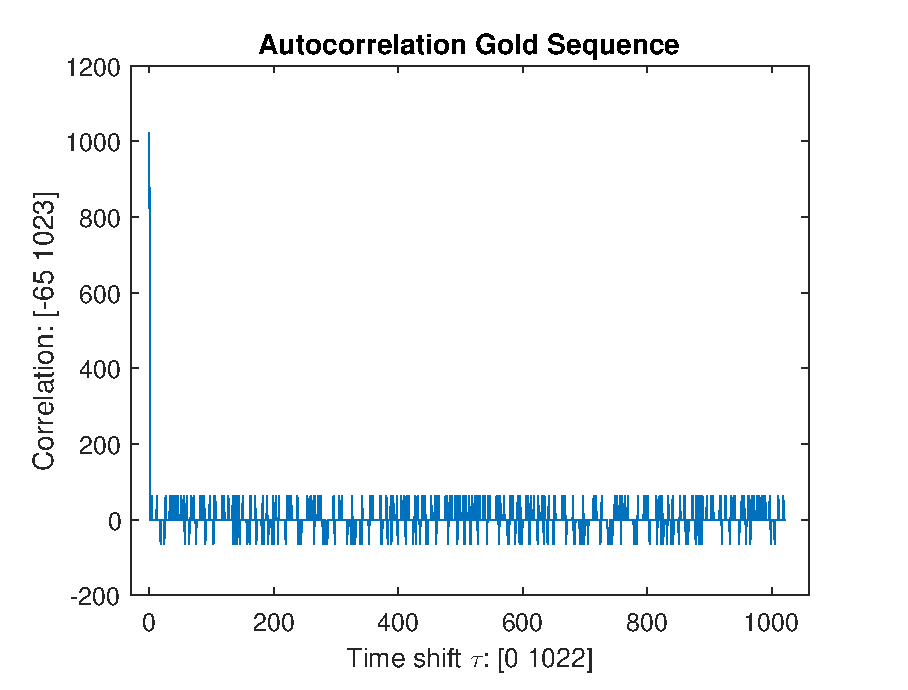
\includegraphics[width=0.9\textwidth]{chapters/cdma-chapters/codes/autocorr-gold.eps}
	\caption{Autocorrelation of one Gold sequence of length 1023.}
	\label{fig:autocorr-gold}
\end{figure}


\begin{figure}[tbp]
	\centering
	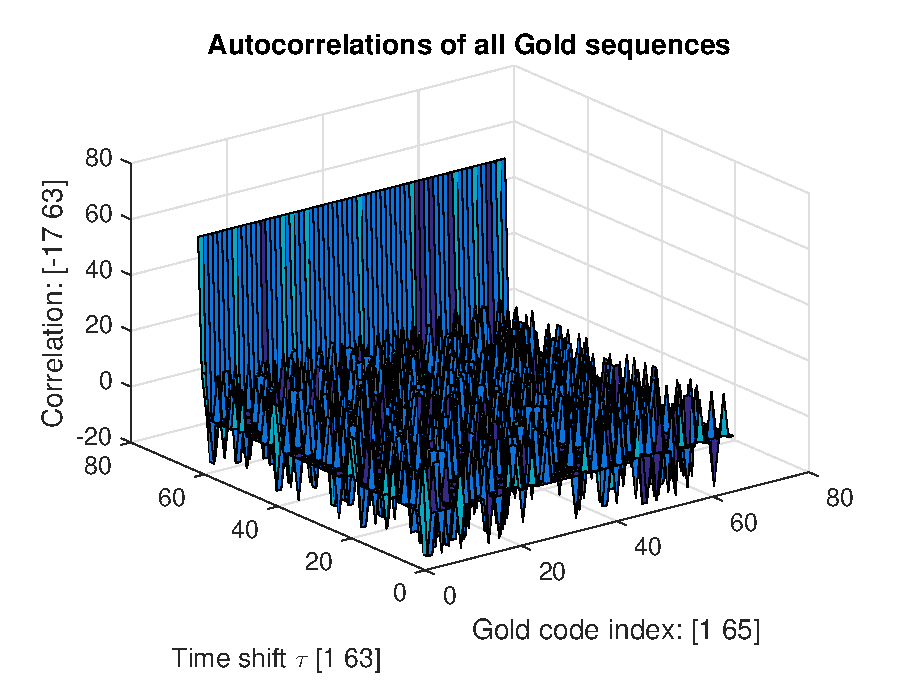
\includegraphics[width=0.9\textwidth]{chapters/cdma-chapters/codes/autocorr-gold-3d.eps}
	\caption{Autocorrelation of all Gold sequences in the same set of length 63.}
	\label{fig:autocorr-gold-3d}
\end{figure}




The autocorrelation properties of Gold sequences are not as good as that of the PN sequences, as can be seen from \autoref{fig:autocorr-gold} compared to \autoref{fig:autocorr-pn}.
The autocorrelation of all the Gold sequences are plotted in \autoref{fig:autocorr-gold-3d} to illustrate that the autocorrelation of all sequences look like each other.
Apart from the original two PN sequences the auto-correlation values can take four values.
The auto-correlation of a PN sequence can be one of two values, see \autoref{eq:autocorr-pn}.
See \autoref{eq:autocorr-gold} and \autoref{eq:gold-t(n)} for the auto-correlation properties of Gold sequences, where $n$ is the length of the LFSR.

\begin{equation}
	\label{eq:autocorr-gold}
	R(\tau) = 
		\begin{cases}
			L    							& \quad \text{if } \tau = 0 \\
			\{ -t(n), \ -1, \ t(n) - 2  \} 	& \quad \text{if } \tau \neq 0 \\
		\end{cases}
\end{equation}

\begin{equation}
	\label{eq:gold-t(n)}
	t(n) = 
		\begin{cases}
			1 + 2^{\frac{n+1}{2}} & \quad \text{for odd } n \\
			1 + 2^{\frac{n+2}{2}} & \quad \text{for even } n \\
		\end{cases}
\end{equation}

See \autoref{eq:corsscorr-gold} and \autoref{eq:gold-t(n)} for the cross-correlation properties of Gold sequences \cite{mitra2008pseudo}.

\begin{equation}
	\label{eq:corsscorr-gold}
	R_{xy}(\tau) = 	\{ -t(n), -1, t(n) - 2  \} 
\end{equation}


From these equations it is clear to see that the absolute maximum cross-correlation is bounded by $t(n)$.
See \autoref{tbl:gold-sequences-C-and-cross-corr} for the cross-correlation for different lengths of Gold sequences.


\begin{table}[tbp]
	\centering
	\begin{tabular}{  | l | l | l | }

		\hline
		Code Length (L)	& Number of Codes (C) 	& Peak cross-correlation ($|t(n)|$)	\\ \hline
		
		7				& 9						& 5						\\ \hline					
		31				& 33					& 9						\\ \hline			
		63				& 65					& 17					\\ \hline			
		127				& 129					& 17					\\ \hline	
		511				& 513					& 33					\\ \hline	
		1023			& 1025					& 65					\\ \hline	

	\end{tabular}
	\caption{Table showing the number of Gold sequences of the same length along with the peak cross-correlation. }
	\label{tbl:gold-sequences-C-and-cross-corr}

\end{table}

As seen from \autoref{tbl:gold-sequences-C-and-cross-corr}, the number of codes scales linearly with the code length, so the gold codes are scalable.
With a LFSR of length $n$, the sequence length is $L = 2^n - 1$ and the number of sequences is $C = 2^n + 1$.
Compared to the peak cross-correlation of the PN sequences, \autoref{tbl:pn-sequences-C-and-cross-corr}, the peak cross-correlation of the Gold sequences are lower for the same code length, see \autoref{tbl:gold-sequences-C-and-cross-corr}.



% Taken out because this is not used anywhere....

%When $n$ is chosen to be odd, something can be said about the approximate frequency of occurrence of the cross-correlation values, see \autoref{tbl:freq-occurence-gold-cross-correlation} \cite{holmes2007spread}.

%\begin{table}[h]
%	\centering
%	\begin{tabular}{ | l | l | }
%
%		\hline
%		$R_{xy}(\tau)$ 	& Frequency of occurrence	\\ \hline
%
%		$-1$			& 0.5					 	\\ \hline
%		$-t(n)$			& 0.25						\\ \hline
%		$t(n) - 2$		& 0.25						\\ \hline
%
%		
%
%	\end{tabular}
%	\caption{Table containing the approximate frequency of occurrence for all the cross-correlation values for $n$ odd.}
%	\label{tbl:freq-occurence-gold-cross-correlation}
%\end{table}



Not all Gold sequences have the balance property that the PN sequences do have.
Roughly half of the sequences in the same set are balanced, sometimes this can be as high as three quarters \cite{holmes2007spread}.


To conclude: The cross-correlations of the Gold sequences are better than those of the PN sequences.
Also the scalability is better and the sequences can still be used for asynchronous transmission.


% !TeX root = ../../../thesis.tex

\subsection{Comparison of Sequences}
\label{subsec:comparison-of-sequences}


In \autoref{tbl:comparison-sequences} a comparison is made between the CDMA sequences discussed.
The sequences are compared for the metrics discussed in \autoref{sec:performance-metrics-cdma} in both synchronous as well as a-synchronous environments.
From this table it is clear that the Gold sequences are the best sequences suited for the environment of disaggregating individual lights, due to their a-synchronous nature, low cross-correlation and one-peaked auto-correlation and their scalability.







\begin{table}[h!]
	\centering
	\begin{tabular}{  | l | l | l | l | }

		\hline
														& Orthogonal Seq. 			& PN Seq.						& Gold Seq.				\\ \hline
		Synchronous	Transmission						& \cmark					& \cmark						& \cmark				\\ \hline
		A-synchronous Transmission						& \xmark					& \cmark						& \cmark				\\ \hline
		Peaks auto-correlation (synchronous)			& 1							& 1								& 1						\\ \hline
		Peaks auto-correlation (a-synchronous)			& $> 1$						& 1								& 1						\\ \hline
		Low cross-correlation (synchronous)				& \cmark					& \cmark						& \cmark				\\ \hline
		Low cross-correlation (a-synchronous)			& \xmark					& \cmark						& \cmark				\\ \hline
		Math. bounded cross-correlation (synchronous)	& \cmark					& \xmark						& \cmark				\\ \hline
		Math. bounded cross-correlation (a-synchronous)	& \xmark					& \xmark						& \cmark				\\ \hline
		Scalability ($C \propto L$)						& \cmark					& \xmark						& \cmark				\\ \hline				



	\end{tabular}
	\caption{Table showing a comparison of the discussed CDMA sequences. }
	\label{tbl:comparison-sequences}

\end{table}

% !TeX root = ../../thesis.tex

\section{Interference Solution}
\label{sec:interference-solution}

In the previous sections, interference was discussed when using a CDMA approach.
When there are too many transmitters on the same channel, at the same time, the interference can be so great that it destroys a code sequence of one or more transmitters.
This is not a problem for Orthogonal sequences, since they have no cross correlation, when transmitted synchronously (See \autoref{sec:orthogonal-sequences}).
But this is an issue for Gold sequences. \todo{Should also mention PN sequences in general, and then the table with the calculated cross correlation per length ????}
As stated in \autoref{subsec:gold-sequences}, the cross correlation of Gold sequences is bounded by $t(n)$, see \autoref{eq:gold-t(n)}.
This means that the maximum number of transmitters can be calculated such that not too much interference will occur. 
With this information two methods can be used to overcome the interference problem.



\subsection{Continuous Method}


One method is to only use so many transmitters in the system that no interference will occur.
A threshold $T$ must be set for which we will accept or reject a correlation as being a valid result.
When a particular code sequence is present in the received signal, the correlation will be equal to the length of the code, $L$.
To prevent false negatives, meaning there is a code sequence present in the received signal but it is lost due to too much interference from other code sequences, the correlation result needs to be higher than the threshold $T$.
The correlation result itself is equal to $R = L + \displaystyle\sum_{t = 0} ^ {L - 1} \Bigg\{ c_0(t) \times  \displaystyle\sum_{i = 1} ^ {m} c_i(t) \Bigg\} $ (See \autoref{sec:mapping-problem}).
Assuming the worst case scenario and each correlation with each other code sequence will be the negative of the absolute maximum cross correlation $t(n)$, the correlation is: $R = L - m \times t(n)$, where $m$ is the number of transmitters.
The correlation needs to be higher than the threshold $T$ to prevent false negatives, so we get the following equation \autoref{eq:gold-max-tx-pt1}.

\begin{equation}
	\label{eq:gold-max-tx-pt1}
	R = L - m \times t(n) > T
\end{equation}

Now to also prevent false positives, meaning there is no code sequence $c_0(t)$ present but due to interference the correlation result suggests that it is present, we get \autoref{eq:gold-max-tx-pt2}.


\begin{equation}
	\label{eq:gold-max-tx-pt2}
	R = m \times t(n) < T
\end{equation}

If we equalize \autoref{eq:gold-max-tx-pt1} and \autoref{eq:gold-max-tx-pt2}, we can calculate what $m$ and $T$ are.
The results can be seen in \autoref{eq:m} and \autoref{eq:T}, respectively.


\begin{equation}
	\label{eq:m}
	m = \frac{L}{2 \times t(n)}
\end{equation}

\begin{equation}
	\label{eq:T}
	T = \frac{L}{2}
\end{equation}


Using the equations above, a table can be compiled showing the maximum number of simultaneous transmitters for which it is guarantied that there will be no false-positives and/or false-negatives when decoding the incoming signal.
The table can be seen in \autoref{tbl:correlation-gold-families}.
 %\cite{holmes2007spread}



\begin{table}[h]
	\centering
	\begin{tabular}{ | l | l | l | l | l |  }

		\hline
		LFSR size (n) 	& Code length (L)	& Number of codes (C)	& Cross-corr. ($|t(n)|$) 	& $m$	\\ \hline

		3				& 7					& 9						& 5							& 0.70	\\ \hline
		%4				& 15				& 17					& 9							& 0.83	\\ \hline %because mod 4 ....
		5				& 31				& 33					& 9							& 1.72	\\ \hline
		6				& 63				& 65					& 17						& 1.85	\\ \hline
		7				& 127				& 129					& 17						& 3.74	\\ \hline
		%8				& 255				& 257					& 33						& 3.86	\\ \hline is not a preferred pair for because mod 4 etc...			
		9				& 511				& 513					& 33						& 7.74	\\ \hline%
		10				& 1023				& 1025					& 65						& 7.87	\\ \hline	%
		%

	\end{tabular}
	\caption{Table containing the maximum number of simultaneous transmitters $m$, such that no destructive interference takes place.}
	\label{tbl:correlation-gold-families}
\end{table}



Because of this value $m$, not all transmitters can transmit continuously.
But if we had a system with a total amount of $m$ transmitters, we could reverse calculate what code length to use such that all transmitters can transmit continuously.
In \autoref{eq:m}, $m$ is written as a function of $n$.
We need $n$ as a function of $m$, so that $L$ can be expressed as a function of $m$.
The length of the code sequence $L$ as a function of the number of simultaneous transmitters $m$ can be found in \autoref{eq:L-f(m)}.
For simplification reasons, the cross correlation function $t(n)$ was taken for $n$ odd. 
The methods used to reverse calculate the equation is beyond the scope of this thesis.


\begin{equation}
	\label{eq:L-f(m)}
	L = \Bigg(\sqrt{2 \times m^2 + 2 \times m + 1} + \sqrt{2} \times m \Bigg)^2 - 1
\end{equation} 


What we can conclude from \autoref{eq:L-f(m)}, is that $L$ is a polynomial function of $m$.
The time $t$ it takes to complete one transmission can be found in \autoref{eq:time-for-m-txs}, where $L$ is length of the code, a function of $m$, the number of simultaneous transmitters, and $f$ is the constant modulating frequency in Hz.
This will guaranty good decoding properties, meaning no false-positives and/or false-negatives and all transmitters can transmit the entire time, simultaneous.
%Also the system is scalable as the time is dependent on a polynomial function of the number of transmitters.

\begin{equation}
	\label{eq:time-for-m-txs}
	t = \frac{L}{f}
\end{equation}


\begin{table}[h]
	\centering
	\begin{tabular}{  | l | l | }

	\hline
	Number of transmitters (m)	& Time (t)					\\ \hline


	%1							& 0.0031 s					\\ \hline
	%3							& 0.0127 s					\\ \hline
	%7							& 0.0511 s					\\ \hline 
	15							& 0.2047 s					\\ \hline
	31							& 0.8191 s					\\ \hline
	63							& 3.2767 s					\\ \hline
	127							& 13.107 s					\\ \hline
	255							& 52.429 s					\\ \hline
	511							& 209.72 s (3.5 min)		\\ \hline
	1023						& 838.86 s (14.0 min)		\\ \hline
	2047						& 3355.4 s (55.9 min)		\\ \hline
	4095						& 13421.7 s (3.7 hour)		\\ \hline
	8191						& 53687.1 s (14.9 hour)		\\ \hline
	16383						& 214748.4 s (2.5 day)		\\ \hline
	32767						& 858993.5 s (1.4 week)		\\ \hline



\end{tabular}
	\caption{Table containing time it takes to receive each transmission from each transmitter, as a function of the number of transmitters, with a constant modulating frequency $f = 10000$ kHz.}
	\label{tbl:continous-method-time-as-function-N}
\end{table}

\autoref{tbl:continous-method-time-as-function-N} states the time needed to receive a transmission from a transmitter as a function of the total number of transmitters in the systems. 
All the other transmitters in the system will also be transmitting at the same time.





\subsection{Probabilistic Method}



Another solution to overcome the interference problem, is to use probabilistic method.
The benefit of this method is that it can utilize all code sequences in the set, instead of a limited amount of them like in the solution above.
The drawback is that it is not guarantied that every transmitter will transmit within a certain time and therefor the time it takes for all transmitters to transmit is not guarantied to be within a certain time frame.


Each transmitter is given the same probability $p$ for which it will transmit and with probability $1 - p$ it will not transmit, which is a Bernoulli distribution.
Since there is more than one transmitter which follows a Bernoulli distribution, the number of transmitters which will be transmitting at any point in time, is a Binomial distribution.
Now that every transmitter has a probability $p$, the following items need to be assessed:

\begin{itemize}
	\item What should $p$ be in order to guaranty, to a certain degree, that the decoding process will not suffer from interference ?
	\item Will every transmitter transmit their code, and if so within what time frame ?
	\item What is the total time for which we can guaranty, to a certain degree, such that every transmitter has transmitter their code at least once ? 
\end{itemize}


\todo{Sources required for the PDF/PMF etc ??}

The probability $p$ must be chosen such that at every point in time the number of transmitters transmitting their sequence will not exceed $m$, in order to not have interference issues.
The cumulative distribution function for a binomial distribution can be seen in \autoref{eq:cdf-binomial}, where $X$ is the random variable for the number of transmitters at every point in time, $m$ is the maximum number of transmitter to avoid interference issues and $N$ is the total number of transmitters used.
The probability that $X \le m$ needs to be as high as possible to avoid the interference issue, but as the CDF goes asymptotically to $1$, we cannot choose the probability $1$.
Instead a value of $1 - \epsilon$ is chosen.
\autoref{eq:cdf-binomial} is then equalized to $1 - \epsilon$ to find a probability $p$, since every other variable is known.
With the found probability $p$, the probability that the number of transmitters at every point in time, PR$(X \le m)$, will not exceed $m$ is equal to $1 - \epsilon$.

\begin{equation}
	\label{eq:cdf-binomial}
	\text{CDF:  PR}(X \le m) = \displaystyle\sum_{i=0}^{m} \binom Ni \times p^i \times (1 - p)^{N-i}
\end{equation}




Since every transmitter transmits their code with probability $p$ there is a probability that it will never transmit its code.
The probability that a transmitter will have transmitted at least once after $k$ attempts, follows a geometric distribution.
%Because each transmitter is independent and identical, the answer to the question holds for every transmitter. 
The CDF of a geometric distribution can be expressed as seen in \autoref{eq:cdf-geometric}, where $Y$ is the number of attempts until the first transmission, $p$ is the probability that the transmitter will transmit and $k$ is the number attempts until the first transmission for which you want to know the probability.
This probability needs to be as high as possible, so that the number of attempts $k$ is as low as possible.
The CDF goes asymptotically to $1$, so we cannot choose $1$, instead $1 - \epsilon_1$ is chosen.
$k$ can now be expressed as can be seen in \autoref{eq:reverse-cdf-geometric}, where $k$ is the number of attempts until the first transmission, $p$ is the probability that the transmitter will transmit and $\epsilon_1$ is a very small number.

\begin{equation}
	\label{eq:cdf-geometric}
	\text{CDF:  Pr}(Y \le k) = 1 - (1 - p)^k
\end{equation}

\begin{equation}
	\label{eq:reverse-cdf-geometric}
	k = \frac{\ln\epsilon_1}{\ln(1 - p)}
\end{equation}

So after $k$ attempts the probability that a transmitter will have transmitted at least once, is $1 - \epsilon_1$.
This holds for one transmitter, but since each transmitter works in parallel and each random variable is independent and identically distributed, this distribution holds for the entire system with $N$ transmitters.
Now the time it takes for all transmitters to transmit at least once, can be calculated.
The result can be seen in \autoref{eq:time-for-probabilistic-txs}, where $L$ is the length of the sequence, $f$ is the constant modulating frequency, $k$ is the number of attempts until the first transmission and $p$ is the probability that a transmitter will transmit.
$L$ and $p$ are effectively functions of $N$, the number of transmitters in the system.

\begin{equation}
	\label{eq:time-for-probabilistic-txs}
	t = \frac{L}{f} \times k = \frac{L}{f} \times \frac{\ln(\epsilon_1)}{\ln(1 - p)}
\end{equation}

This probabilistic method allows to use all the sequences in the same set.
The drawback is that the time frame for which all transmitters have transmitted, is dependent on the values that are set for $\epsilon$ and $\epsilon_1$.
In \autoref{tbl:probabilistic-method-time-as-function-N} the time it takes to let each transmitter transmit at least once, is listed as a function of the number of transmitters in the total system. 
When both the epsilons are quite small, $\epsilon = \epsilon_1 = 0.001$, the probability of interference is small, but the times grow larger.
For $\epsilon = \epsilon_1 = 0.1$, the times are smaller, but the probability of interference will be higher.
A simulation is needed in order to asses if this will give acceptable results.
\todo{Prob. do a simulation for this in the eval. sections and reference it.}



\begin{table}[h]
	\centering
	\begin{tabular}{  | l | l | l | }

		\hline
		Number of transmitters (N)	& Time (t), $\epsilon = \epsilon_1 = 0.001$	& Time (t), $\epsilon = \epsilon_1 = 0.1$		\\ \hline

		9							& 43.5 s									& 0.1 s 										\\ \hline
		33							& 15.3 s									& 0.4 s											\\ \hline
		65							& 14.6 s									& 0.8 s											\\ \hline
		129							& 26.1 s									& 2.1 s											\\ \hline
		513							& 91.3 s (1.5 min)							& 12.9 s										\\ \hline
		1025						& 178.2 s	(3.0 min)						& 30.7 s										\\ \hline
		2049						& 450.8 s	(7.5 min)						& 86.4 s (1.4 min)								\\ \hline
		8193						& 2672.4 s (44.5 min)						& 617.0 s (10.3 min)							\\ \hline
		16385						& 6651.4 s (1.8 hour)						& 1644.0 s (27.4 min)							\\ \hline
		32769						& 17616.9 s (4.9 hour)						& 4577.2 s (1.3 hour)							\\ \hline


	\end{tabular}
	\caption{Table containing time it takes to let each transmitter transmit at least once, as a function of the number of transmitters, with a constant modulating frequency $f = 10000$ kHz.}
	\label{tbl:probabilistic-method-time-as-function-N}
\end{table}

%\begin{table}[h]
%	\centering
%	\begin{tabular}{ | l | l | l | l | }
%
%		\hline
%		LFSR size (n) 	& Number of transmitters (N)	& Time (t), $\epsilon = \epsilon_1 = 0.001$	& Time (t), $\epsilon = \epsilon_1 = 0.1$		\\ \hline
%
%		3				& 9								& 43.5 s									& 0.1 s 										\\ \hline
%		%4				& 17							& 											& 												\\ \hline
%		5				& 33							& 15.3 s									& 0.4 s											\\ \hline
%		6				& 65							& 14.6 s									& 0.8 s											\\ \hline
%		7				& 129							& 26.1 s									& 2.1 s											\\ \hline
%		9				& 513							& 91.3 s (1.5 min)							& 12.9 s										\\ \hline
%		10				& 1025							& 178.2 s	(3.0 min)						& 30.7 s										\\ \hline
%		11				& 2049							& 450.8 s	(7.5 min)						& 86.4 s (1.4 min)								\\ \hline
%		13				& 8193							& 2672.4 s (44.5 min)						& 617.0 s (10.3 min)							\\ \hline
%		14				& 16385							& 6651.4 s (1.8 hour)						& 1644.0 s (27.4 min)							\\ \hline
%		15				& 32769							& 17616.9 s (4.9 hour)						& 4577.2 s (1.3 hour)							\\ \hline
%
%
%	\end{tabular}
%	\caption{Table containing time it takes to let each transmitter transmit at least once, as a function of the number of transmitters.}
%	\label{tbl:time-as-function-N}
%\end{table}






% !TeX root = ../../thesis.tex

\section{Mapping Problem}
\label{sec:mapping-problem}

The coding methods as discussed in \autoref{subsec:orthogonal-sequences} and \autoref{subsec:pn-sequences} are used in the field of telecommunication.
Since these signals are analog radio waves, the symbols are $+1$ and $-1$ and they are balanced around $0$.
The LFS registers used with the generation of PN and gold sequences, only output zeros and ones.
For the use with radio-signals a code sequence is mapped to a form with $+1$ and $-1$, where the original $0$ is mapped to $+1$ and the original $1$ is mapped to $-1$ \cite{cdma-mapping-symbols-ref}.



First the equations are shown, how to calculate the correlation for a particular code when the code sequences from all the transmitters only have $+1$ and $-1$ symbols. 
In \autoref{eq:eqns-correlation-normal-symbols} it is shown how to calculate the correlation $R$, where we use \autoref{eq:correlation} and where $s(t)$ is the received signal which is the composed signal of $m$ distinct codes, which all use the $+1$ and $-1$ symbols and where $c^r_1(t)$ is the code sequence, with symbols $+1$ and $-1$, for which we want to calculate the correlation.


\begin{equation}
	\begin{array}{l}
		R_{sc^r_{1}} = \displaystyle\sum_{t = 0} ^ {L - 1} s(t) \times c^r_1(t)	 \\
		s(t) = \displaystyle\sum_{i = 1} ^ {m} c^r_i(t) \\
		R_{sc^r_{1}} = \displaystyle\sum_{t = 0} ^ {L - 1} \Bigg\{ c^r_1(t) \times  \displaystyle\sum_{i = 1} ^ {m} c^r_i(t) \Bigg\} 
	\end{array} 
	\label{eq:eqns-correlation-normal-symbols}
\end{equation}


%The following proof \todo{Are we calling this a proof ??} shows how to calculate the correlation when the coding sequence consists of $+1$ and $-1$ symbols: 

%\begin{proof}
%	Let $s(t)$ be the received signal which is the composed signal of $m$ distinct codes.\\
%	And let $c_i(t)$ be the code sequence $i$, and let $c_1(t)$ be the code for which we want to check if there is information there. \\
%
%	\begin{align*}
%		R(\tau)_{xy} = \displaystyle\sum_{t = 0} ^ {L - 1} x(t) \times y(t + \tau)	\tag{See \autoref{eq:correlation}}
%		\\ \tau = 0,\ x = s(t),\ y = c_1(t)	
%		\\ R(0)_{sc_{1}} = \displaystyle\sum_{t = 0} ^ {L - 1} s(t) \times c_1(t)
%		\\ s(t) = \displaystyle\sum_{i = 1} ^ {m} c_i(t)														
%		\\ R(0)_{sc_{1}} = \displaystyle\sum_{t = 0} ^ {L - 1}  \Bigg\{  c_1(t)	\times \displaystyle\sum_{i = 1} ^ {m} c_i(t) \Bigg\}
%		\\ R(0)_{sc_{1}} = \displaystyle\sum_{t = 0} ^ {L - 1} \Bigg\{ c_1(t) \times c_1(t) + c_1(t) \times  \displaystyle\sum_{i = 2} ^ {m} c_i(t) \Bigg\} 
%		\\ R(0)_{sc_{1}} = \displaystyle\sum_{t = 0} ^ {L - 1} c_1(t) \times c_1(t) + \displaystyle\sum_{t = 0} ^ {L - 1} \Bigg\{ c_1(t) \times  \displaystyle\sum_{i = 2} ^ {m} c_i(t) \Bigg\} 
%		\\ R(0)_{sc_{1}} = L + \displaystyle\sum_{t = 0} ^ {L - 1} \Bigg\{ c_1(t) \times  \displaystyle\sum_{i = 2} ^ {m} c_i(t) \Bigg\} 
%	\end{align*}

%\end{proof}

The correlation calculation holds for any sequence with $+1$ and $-1$ symbols.
For example: Assume $c^r_1 = \{ -1, 1, -1, -1, -1 \}$ and $c^r_2 = \{ 1, -1, -1, 1, -1 \}$.
Note that code $c^r_1$ is not balanced, the sum is equal to $-3$, code $c^r_2$ is balanced because the sum is equal to $-1$.
Also note that these sequences are completely chosen at random, the codes are not orthogonal, pn or gold sequences.
These codes are the IDs of transmitters 1 and 2, respectively.
Also assume that these codes are transmitted at the same time to create $s = c^r_1 + c^r_2 = \{ 0, 0, -2, 0, -2 \}$.
The calculated correlation using \autoref{eq:eqns-correlation-normal-symbols} will now be: $R_{sc^r_{1}} = 4$ and $R_{sc^r_{2}} = 4$.
These are the correlation results when codes are used with $+1$ and $-1$ symbols.
%This example will be used again later in this section to compare when different symbols are used.

The result of \autoref{eq:eqns-correlation-normal-symbols} is the sum of all the correlations. 
If the code that is being correlated with, is present in the signal $s(t)$ then one of the outcomes of the correlation will be the peak auto-correlation $L$ then we can write the total correlation as follows: $R_{sc_{1}} = L + \displaystyle\sum_{t = 0} ^ {L - 1} \Bigg\{ c_1(t) \times  \displaystyle\sum_{i = 2} ^ {m} c_i(t) \Bigg\} $, where the result is the auto-correlation $L$ plus all the other correlations.
If the orthogonal sequences were used all the other correlations are zero.
If the Gold sequences were used each of the other correlations could be one of the values as stated in \autoref{eq:corsscorr-gold}.
This is where the multiple access interference shows.







The above correlation calculation only holds, when using a coding sequence which has $+1$ and $-1$ symbols.
However, for the states of the LEDs we can only choose between an on or off state with OOK, so a $1$ or a $0$.
This means a different correlation calculation is required.
First a formula for the mapping from $+1$ to zero and $-1$ to one is needed.
The formula can be found in \autoref{eq:radio-to-bin}, where $r$ denotes the $+1$ or $-1$ symbols and the outcome $b$ will be our binary value, $0$ or $1$.
This mapping formula is based on the mapping used by PN sequences to work with wireless communication
A PN sequence outputs zeros and ones and these are mapped to $+1$ and $-1$ respectively \cite{cdma-mapping-symbols-ref}.
 
\begin{equation}
	b = \frac{1 - r}{2}
	\label{eq:radio-to-bin}
\end{equation}


The codes that were used in the example above, can now be mapped to $0$ and $1$ symbols.
This results in the following codes: $c^b_1 = \{ 1, 0, 1, 1, 1 \}$ and $c^b_2 = \{ 0, 1, 1, 0, 1 \}$.
The $b$ notation indicates that these sequences consists of $0$ and $1$ symbols.



The previous equation (\autoref{eq:eqns-correlation-normal-symbols}) can now be altered to incorporate the fact that the LEDs work with a one and zero state.
In \autoref{eq:eqns-correlation-binary-symbols} it is shown how the correlation formula changes when the codes that are used for the LEDs now have $0$ and $1$ values instead of the $+1$ and $-1$ values.
In \autoref{eq:eqns-correlation-binary-symbols} the new correlation $\hat{R}$ is calculated, where $c^r_i(t)$ is the code sequence $i$ and consists of symbols $-1$ and $+1$, and $c^b_j(t)$ is the code sequence $j$ and consists of symbols $1$ and $0$ and where $s(t)$ is the received signal which is the composed signal of $m$ distinct codes.
To clarify: The codes that the LEDs use have values $0$ and $1$ due to the OOK, the code that is being correlated with at the receiver or current-sampler side still uses the $+1$ and $-1$ symbols.








The altered correlation calculation, denoted by $\hat{R}$ shows different results than the previous result $R$.
Where $R_{sc_{1}} = \displaystyle\sum_{t = 0} ^ {L - 1} \Bigg\{ c^r_1(t) \times  \displaystyle\sum_{i = 1} ^ {m} c^r_i(t) \Bigg\} $ and $\hat{R}_{sc^r_{1}} = \frac{m}{2} \times \displaystyle\sum_{t = 0} ^ {L - 1} c^r_1(t) - \frac{1}{2} \times \displaystyle\sum_{t = 0} ^ {L - 1}  \Bigg\{ c^r_1(t) \times \displaystyle\sum_{i = 1} ^ {m} c^r_i(t) \Bigg\}$.
We can write it such that $R$ will become a function of $\hat{R}$ as can be seen in \autoref{eq:final-mapped-correlation-function}.
With this equation we get the same output domain as with the normal correlation formula used for the codes that have $+1$ and $-1$ symbols.

\begin{equation}
	\begin{array}{l}
		\hat{R}_{sc^r_{1}} = \displaystyle\sum_{t = 0} ^ {L - 1} s(t) \times c^r_1(t)	 \\
		s(t) = \displaystyle\sum_{i = 1} ^ {m} c^b_i(t) = \displaystyle\sum_{i = 1} ^ {m} \frac{1 - c^r_i(t)}{2} \\
		\hat{R}_{sc^r_{1}} = \displaystyle\sum_{t = 0} ^ {L - 1} \Bigg\{  c^r_1(t)	\times \displaystyle\sum_{i = 1} ^ {m} \frac{1 - c^r_i(t)}{2}  	\Bigg\} \\
		\hat{R}_{sc^r_{1}} = \frac{m}{2} \times \displaystyle\sum_{t = 0} ^ {L - 1} c^r_1(t) - \frac{1}{2} \times \displaystyle\sum_{t = 0} ^ {L - 1}  \Bigg\{ c^r_1(t) \times \displaystyle\sum_{i = 1} ^ {m} c^r_i(t) \Bigg\}
	\end{array} 
	\label{eq:eqns-correlation-binary-symbols}
\end{equation}



\begin{equation}
	R_{sc^r_{1}} = m \times \displaystyle\sum_{t = 0} ^ {L - 1} c^r_1(t) - 2 \times \hat{R}_{sc^r_1}
	\label{eq:final-mapped-correlation-function}
\end{equation}


When the transmitters or LEDs in this case, transmit the codes $c^b_1$ and $c^b_2$, the following signal $s$ would be created: $s = c^b_1 + c^b_2= \{ 1, 1, 2, 1, 2 \}$.
\autoref{eq:eqns-correlation-binary-symbols} can now be used to calculate the new correlation $\hat{R}$: $\hat{R}_{sc^r_{1}} = -5$ and $\hat{R}_{sc^r_{2}} = -3$.
These results are not the same as with the previous correlation results, where the results were 4 and 4, respectively.
This is because $R$ and $\hat{R}$ cannot be compared, instead the results obtained from $\hat{R}$ need to be mapped to $R$.
The values obtained using $\hat{R}$ can now be mapped to $R$ by using \autoref{eq:final-mapped-correlation-function}. %($\hat{R}_{sc^r_{1}} = -5$ and $\hat{R}_{sc^r_{2}} = -3$)
For this equation we also need the sum of the code sequences, which were already calculated in the beginning of the example to show that one of the code sequences is not balanced.
The sums are: $\displaystyle\sum c^r_1 = -3$ and $\displaystyle\sum c^r_2 = -1$.
To obtain $R$: $R_{sc^r_{1}} = m \times \displaystyle\sum c^r_1 - 2 \times \hat{R}_{sc^r_1}  = 2 \times -3 - 2 \times -5 = 4$ and $R_{sc^r_{2}} = m \times \displaystyle\sum c^r_2 - 2 \times \hat{R}_{sc^r_2} = 2 \times -1 -2 \times -3 = 4$.
And these correlation results are the same as the correlation results as with the codes which had $-1$ and $+1$ symbols.
Hence, we show that any sequence can be mapped from $-1$ and $+1$ symbols to $0$ and $1$ symbols and still get correct correlation results.




In \autoref{eq:final-mapped-correlation-function} the sum of the sequence used to correlate with, is needed. 
The sum of the sequence depends on the sequence used, when using orthogonal codes the sum will be zero, see \autoref{subsec:orthogonal-sequences}.
If the sum is equal to zero, the factor $m$ will not matter.
However when the sequence used is a PN sequence or a balanced Gold sequence, the sum will be $-1$.
The sum will be $-1$ due to the fact of the balance property of the PN sequences, as explained in \autoref{subsec:pn-sequences}.
The sequence will have exactly $2^{n-1}$ ones, where the ones will be mapped to $-1$ and the sequence will have exactly $2^{n-1} -1$ zeros, which will be mapped to $1$.
These mappings can be found when inversing \autoref{eq:radio-to-bin}, this yields: $r = 1 - 2 \times b$.
When we calculate the sum of the sequence we get: $2^{n-1} \times -1 + (2^{n-1} - 1) \times 1 = -1$.
Because the sum is equal to $-1$: $R = -m - 2 \times \hat{R}$, and then $m$, the number of signals, is important.
When using an unbalanced Gold sequence, the sum of that sequence is not equal to $-1$.
All the chips of the unbalanced Gold sequence can be added, in order to find the sum of this particular sequence and use the outcome to calculate the correct correlation value as we have done for the example with code $c^r_1$.











